\infolevone{
\section{Beam Current Measurement}
-%\setcounter{subsection}{0}

%%% This is lifted from the Hall A manual

The Beam Current Monitor (BCM) is designed for stable, low noise,
non-intercepting beam current measurements. The primary system
consists of an Unser monitor and two rf cavities (bcm1 and bcm2), with
associated electronics and a data acquisition system. An additional
three RF cavities are also available for use for most experiments,
although must be removed for certain configurations of the beamline
(e.g. during polarized target experiments that require a slow raster
system). There is also a bcm (bcm17) placed upstream of the Hall C
Compton polarimeter on the 3C17 girder. This bcm is used primarily for
current measurements for the Hall C polarimeters.  The Unser monitor,
bcm1, and bcm2 are wrapped in thermal blankets for temperature
stabilization and are located 7.7 meters upstream of the target. The
additional rf cavity triplet is enclosed in a thermally stabilized box
and is located at the end of the blue platform that extends from the
Hall C beam way, about 13 meters upstream of the target. In the
standard configuration, an additional bcm is placed immediately
upstream of the target; this bcm is controlled/read out for purposes
of machine protection (to monitor beam loss) and is not considered
part of the Hall C current measurement system for experiments.

All electronics for reading out the Hall C bcms, as well as the
temperature controllers, are located in the Counting House.

%The readout chain is slightly different for the different sets of
%bcms. The rf cavities on the Unser girder (bcm1 and bcm2) are readout using a 100 kHz
%analog down converter and an RMS to DC converter. The resulting DC signal is sent through a pre-amplifier
%and on to a V2F module for readout of the bcm signals in scalers.  Optimal linearity for a given
%current range is achieved by manual adjustment of an analog amplifier placed between the down converter
%and the RMS to DC converter.  The current monitors on the blue platform
%(bcma, bcmb, and bcmc) are read out using a digital down converter with onboard ADC, FPGA, and DAC. This module
%provides a DC signal which can then be either sent to V2Fs or an ADC for use in the data acquisition. These
%electronics (in particular, the system gain settings) are controlled via an EPICS interface.

\subsection{System Layout}

The schematic diagram of the BCM system is presented in
Fig.~\ref{fig:hallc_bcm}.
\begin{figure}[h!]
\begin{center}
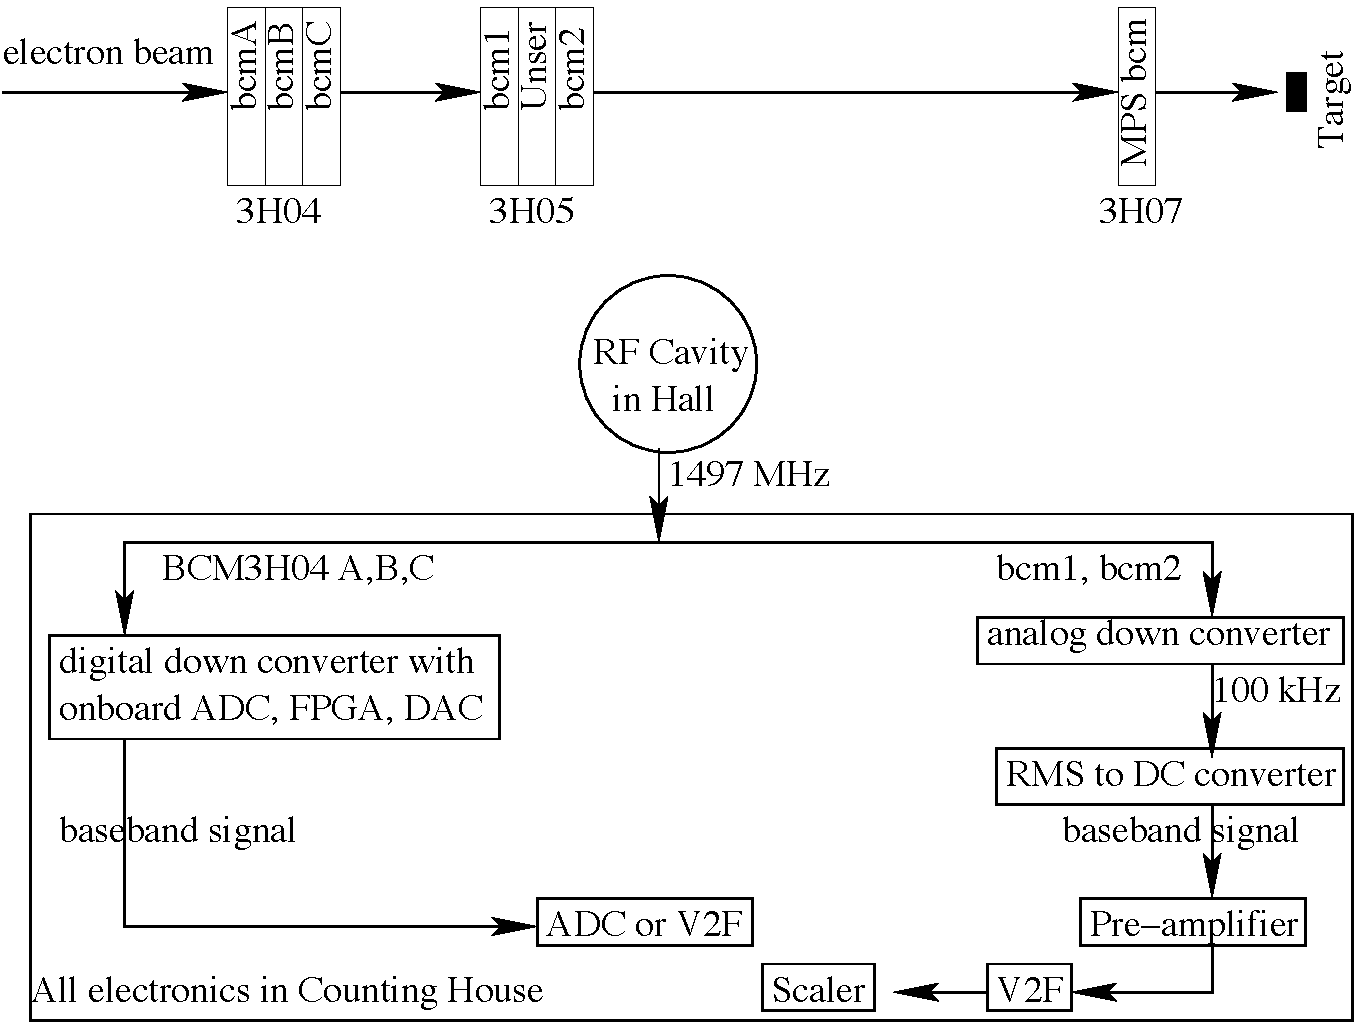
\includegraphics[angle=0,width=15cm]{bcm_electronics.pdf}
\caption[Beam Current Measurement: Schematic]{Schematic of the Hall C beam
current measurement system.}
\label{fig:hallc_bcm}
\end{center}
\end{figure}

The Unser monitor is a Parametric Current Transformer designed for
non-destructive beam current measurement and providing an absolute
reference. The monitor is calibrated by passing a known current
through a wire inside the beam pipe and has a nominal output of 4
mV/$\mu $A. It requires extensive magnetic shielding and temperature
stabilization to reduce noise and zero drift. As the Unser monitor's
output signal drifts significantly on a time scale of several minutes,
it cannot be used to continuously monitor the beam current. However,
this drift is measured during the calibration runs (by taking a zero
current reading) and removed in calibrating the cavities.  The more
stable cavities are then used to determine the beam current and charge
for each run.

The two resonant rf cavity monitors on either side of the Unser
Monitor (bcm1 and bcm2) are stainless steel cylindrical high Q ($\sim
500$) waveguides which are tuned to the frequency of the beam (1.497
GHz) resulting in voltage levels at their outputs which are
proportional to the beam current. Each of the rf output signals from
the two cavities are sent upstairs to the counting house where the rf
output is converted to 100 kHz signals (by the ``downconverters'') and
fed into an RMS-to-DC converter board consisting of a 20 kHz bandpass
filter to eliminate noise, amplified and sent to a V2F (via a
pre-amplifier which adds a 2.5 V offset).  The amplification of the
RMS-to-DC converter is manually adjustable to provide optimal
linearity for the relevant beam current range.  The output of the V2F
modules is sent to the data acquisition for fast readout in scalers. A
copy of the V2F output is also sent to a nearby slow-controls VME
crate for processing and integration into the slow EPICS data stream.

The bcm triplet further upstream of the Unser/bcm1/bcm2 girder (bcma,
bcmb, and bcmc), as well as bcm17, make use of rf cavities of the same
geometry and properties as bcm1 and bcm2. In this case, however, the
readout scheme is a bit different. the rf signals from bcma,bcmb, and
bcmc are sent to the counting house where they are processed using a
digital down converter with onboard ADC, FPGA, and DAC. This module
provides an analog signal which can be sent to an ADC or V2F for
integration in the data acquisition. The readout electronics are
controlled via EPICS (in particular the gain settings), and can also
provide direct EPICS readout.

Absolute calibration of the rf cavities with uncertainties of
100-200~nA is possible depending on how much time is devoted to
calibration with respect to the Unser monitor.

\begin{safetyen}{0}{0}
\subsection{Safety Information}
In coordination with the Hall C run coordinator, all Hall C members
are authorized to take BCM calibration data using the Standard
Non-Invasive Hall C BCM Calibration Procedure which is maintained in
the accelerator document database and it is executed by operates.

\obsolete{
The Accelerator EES group performs the maintenance of the BCM monitors. These 
include:

\begin{tabular}{l l}
1. The Unser calibration. & Every 3 months \\
2. Resonant Cavities Tuning. & Every Downtime \\
3. Multi-meters Autocalibration. & Every Downtime \\
4. Connectors Cleaning. &  Every year \\
5. Unser Keithley Current Source. & Calibration Yearly \\
6. Digital Multi-meters HP3458A and HP 34401A. & Calibration Yearly\\   
\end{tabular}
}

\subsubsection{Hazards and Mitigations}

As operators perform the calibration procedures there is no hazard to
Hall C personnel in performing a beam current measurement.

\subsubsection{Responsible Personnel}
System responsible personnel are shown in Table~\ref{tab:BCM:personnel}.
\begin{namestab}{tab:BCM:personnel}{BCM: authorized personnel}{%
   Beam Current Monitor: authorized personnel}
  \DaveMack{\em Contact}
  \JohnMusson{Accel. expert}
\end{namestab}
\end{safetyen}
%Jean-Claude Denard -x 7555

%%% The following is from the old Hall C manual
% There are more BCMs than in the past.  Should these be described too?

%\subsubsection{Ion Chamber} This device will provide an absolute measurement of
%the current at low currents. It has not yet been installed but will reside
%in front of the Hall~C beam dump.

%All questions concerning beam current measurements should be
%directed to Dave Mack - x7442.
}%\infolevone
